\begin{center}
\Huge
Eksponentiel regression
\end{center}
\stepcounter{section}
Vi husker på, at en eksponentiel funktion er en funktion på formen
\begin{align*}
f(x) = b\cdot a^x,
\end{align*}
hvor $a,b>0.$ Eksponentiel vækst kan se ud på forskellige måder. Der skældnes generelt mellem to tilfælde: $a>1$ og $1>a>0$ (Hvad sker der, hvis $a=1$?). Disse to tilfælde fremgår af Fig. \ref{fig:eksp}.
\begin{figure}[H]
\centering
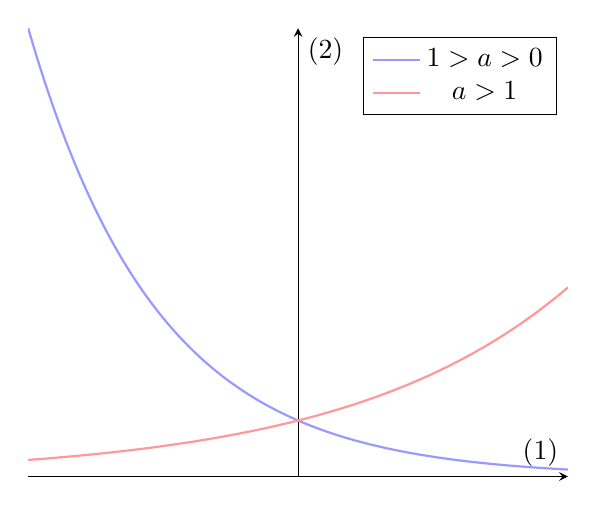
\begin{tikzpicture}
\begin{axis}[axis lines=middle, ticks = none,
ymin = 0,
xlabel = (1),
ylabel = (2)]
\addplot[color=blue!40,thick, domain=-3:3, samples=1000]{2*0.5^x};
\addplot[color=red!40,thick, domain=-3:3, samples=1000]{2*1.5^x};
\legend{$1>a>0$,$a>1$}
\end{axis}
\end{tikzpicture}
\caption{Eksponentiel vækst i de to tilfælde, at $1>a>0$ og $a>1$.}
\label{fig:eksp}
\end{figure}

\section*{Eksponentiel regression}

Vi har tidligere arbejdet med lineær regression af et datasæt. Dette bruger vi, når vi forventer at datasættet kan beskrives af en sammenhæng af typen
\begin{align*}
	f(x) = ax+b.
\end{align*}

I tilfældet at vi antager, at datasættet kan beskrives ved en sammenhæng af typen 
\begin{align*}
	g(x) = b\cdot a^x, 
\end{align*}
så skal vi bruge et andet værktøj - eksponentiel regression. 


\begin{exa}
Af Tab. \ref{tab:1} fremgår et datasæt, der beskriver sammenhængen mellem antallet af bakterier i en petriskål og tiden, der er forløbet.
\begin{table}[H]
	\centering
	\begin{tabular}{c|c|c|c|c|c|c|c}
		$t$ (tid i timer) & 0 & 5 & 10 & 15 & 20 & 25 & 30\\
		\hline
		$B$ (Antal bakterier) & 3.99 & 4.71 & 9.63 & 15.13 & 13.77 & 30.84 & 29.20
	\end{tabular}
	\caption{Sammenhæng mellem forløbet tid $t$ (i timer) og antal bakterier $B$ (i mia.)}
	\label{tab:1}
\end{table}

Vi laver eksponentiel regression i Maple ved at skrive følgende.
\begin{align*}
	&\texttt{with(Gym):}\\
	&\texttt{X:=[0,5,10,15,20,25,30]}\\
	&\texttt{Y:=[3.99,4.71,9.63,15.13,13.77,30.84,29.20]}\\
	&\texttt{ExpReg(X,Y)}
\end{align*}

Resultatet af regressionen kan ses af Fig. \ref{fig:regres}.
\begin{figure}[H]
	\centering
	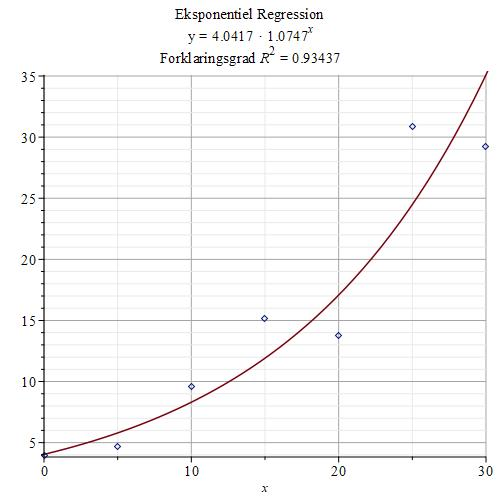
\includegraphics[width=0.7\textwidth]{Billeder/EkspReg.jpg}
	\caption{Eksponentiel regression på datasæt.}
	\label{fig:regres}
\end{figure}
Den eksponentialfunktion $B$, der bedst passer på datasættet er derfor
\begin{align*}
	B(t) = 4.0417\cdot 1.0747^t
\end{align*}

\end{exa}

\section*{Opgave 1}

I \href{https://github.com/ChristianJLex/TeachingNotes/raw/master/2022-2023/Data%20og%20lign/Befolkningsdata.xlsx}{\color{blue!60} dette datasæt} fremgår sammenhængen mellem antallet af personer i en by (i tusinde) fra år 1900 til år 2000.

\begin{enumerate}[label=\roman*)]
	\item Anvend eksponentiel regression på datasættet, der beskriver antallet af personer i byen.
	\item Brug din eksponentialregression til at bestemme antallet af personer, der vil være i år 2010 ifølge modellen.
	\item Afgør, hvornår der vil være 150.000 personer i byen ifølge modellen. 
\end{enumerate}


\section*{Opgave 2}
To biologistuderende har brugt absorbansen af en væske til at måle antallet af bakterier i væsken. De antager, at sammenhængen mellem den forløbne tid (i minutter) og antallet af bakterier (i mia.) kan beskrives ved en eksponentiel sammenhæng. Deres data kan findes \href{https://github.com/ChristianJLex/TeachingNotes/raw/master/2022-2023/Data%20og%20lign/Bakteriedata.xlsx}{\color{blue!60} her}.

\begin{enumerate}[label=\roman*)]
	\item Lav eksponentiel regression og lineær regression på datasættet.
	\item Lav en kvalitativ vurdering af de to modeller. Hvilken virker til at være bedst?
	\item Sammenlign forklaringsgraderne for de to modeller. Hvilken en er bedst? Tror du, at forklaringsgrader kan bruges til at sammenligne forskellige regressionsmodeller?
	\item Brug din valgte model til at afgøre, hvornår der vil være 1 bio. bakterier i væsken. 
\end{enumerate}

\section*{Opgave 3}
8 kg af en radioaktiv isotop placeres på en vægt i år 1810 og vægten nedskrives hvert år indtil år 2010. Vægten af isotopen (i kg) sammen med den passerede tid fremgår af \href{https://github.com/ChristianJLex/TeachingNotes/raw/master/2022-2023/Data%20og%20lign/Isotopdata.xlsx}{\color{blue!60} dette datasæt}.

\begin{enumerate}[label=\roman*)]
	\item Lav eksponentiel regression på datasættet.
	\item Hvor meget vil isotopen veje i år 2050 ifølge modellen.
	\item Hvornår er vægten af isotopen halveret?
	\item Hvis vi antager, at isotopen er helt væk efter 10 halveringstider, hvornår er isotopen så væk?
\end{enumerate}
